We parameterize the amplitudes in the Cartesian space $(b_L,b_T)$ rather than in the Lorentz-invariant variables $(P\cdot b,b^2)$, which are related by $b_L=(P\cdot b)/(-P_L)$ and $b_T^2=b^2-b_L^2$. Because $b^2=b_L^2+b_T^2$, several combinations of longitudinal and transverse separation give the same $b^2$. Fitting directly in $(P\cdot b,b^2)$ would merge these points and reduce the number of data points. We therefore fit in $(b_L,b_T,\eta)$ and transform to the invariant variables in the analysis. The momentum $P_L=-1$ is far from the limit $\hat\zeta\to\infty$ and does not enter the extrapolation of Sec.~\ref{sec:extrapolation}. We therefore determine the model from the data at $P_L=-2$ and fit the same model at the higher momenta.

\subsection{Failure of the Gaussian model and data selection}
\label{sec:fit_strategy}

For the real parts of the amplitudes, Hermitian conjugation requires the function to be even in the longitudinal separation $b_L$ (Eq.~\eqref{eq-ReIm-parity}). We first model the real amplitude with a 2D Gaussian centered at the origin, $\tAmp^{\text{Re}}_{iB}=\gamma\exp[-\alpha b_L^2-\beta b_T^2]$. With $b_T^2=b^2-b_L^2$ and $b_L=(P\cdot b)/(-P_L)$ it becomes $\gamma\exp[-\tfrac{\alpha-\beta}{P_L^2}(P\cdot b)^2-\beta b^2]$ in the invariant variables. For the Fourier integral over $P\cdot b$ to converge, the exponent must remain negative as $P\cdot b\to\pm\infty$, which requires $\alpha>\beta$. If $\alpha<\beta$, the amplitude grows exponentially at large longitudinal separation and the integral diverges. Fitting this Gaussian at $\eta=8$ to all $66$ points, with the correlated $\chi^2$ of the full Jackknife covariance matrix, gives $\alpha<\beta$ for $\tAmp^{\text{Re}}_{2B}$, with $\alpha-\beta=-0.474(5)$ and $\chi^2/\text{dof}=93.9(2.4)$. For $\tAmp^{\text{Re}}_{12B}$ we find $\alpha-\beta=0.005(30)$ with $\chi^2/\text{dof}=2.39(39)$, which is compatible with zero. The Gaussian therefore describes the data poorly and does not allow a convergent Fourier transform. Gaussian ansätze with $\eta$-dependent widths, fitted to all $\eta$ at once, also describe $\tAmp^{\text{Re}}_{2B}$ worse than the Lorentzian power law of Sec.~\ref{sec:power_law} (Sec.~\ref{sec:eta_dependence}).


The Gaussian fit includes quark separations at short distance as well as in the medium range. The short-distance regime, $|\vect{b}|\sim a$ or $2a$, is dominated by perturbative effects, including short-distance divergences that require additional renormalization, and by discretization artifacts. We target the medium-range nonperturbative TMD physics and therefore keep only the data with $|\vect{b}|\ge 3a$.

We also fix the staple extent. The generalized Sivers shift for SIDIS and DY corresponds to $\eta\to\infty$. The first-moment ($x$-integrated) calculation of Ref.~\cite{Musch:2011er} shows that the Sivers shift ratio reaches an asymptotic plateau for $|\eta v|=7a\ldots12a$. The Sivers and unpolarized TMDs are therefore expected to share a common $\eta$ profile that cancels in the asymptotic limit. We include the relatively large range $6\le\eta\le10$ in all global fits in $(b_L,b_T,\eta)$.

\subsection{Symbolic regression with PySR}
\label{sec:pysr}

We use symbolic regression as an aid to explore the functional form of the lattice amplitudes. Unlike traditional regression, which optimizes the parameters of a pre-determined function, symbolic regression searches the space of mathematical expressions and their parameters simultaneously. We use \texttt{PySR}~\cite{Cranmer2023pysr}, a framework that uses genetic programming to discover interpretable equations from data by balancing accuracy and simplicity. It evolves mathematical expressions represented as binary trees and evaluates a population of expressions against the lattice data with a custom loss function. The operator library includes a custom Lorentzian-type binary operator, $\text{lor}(x,y)=1/(1+x^2+y^2)^2$, alongside standard arithmetic and exponential functions, and nesting constraints prevent double-exponential structures. We search for $\tAmp_{2B}^{\text{Re}}(\eta,b_L,b_T)$ with $|\vect b|\ge3a$ and $6\le\eta\le10$.

Standard symbolic regression optimizes metrics like the mean squared error. A genetic algorithm might then discover a polynomial or a diverging exponential function that fits the finite $(b_L,b_T)$ lattice grid well but diverges as $b_L\to\infty$, which makes the Fourier transform over $P\cdot b$ diverge. We therefore implemented a custom loss function that enforces the required asymptotic decay,
\begin{equation}
\mathcal L=\frac{\chi^2}{\text{dof}}+\epsilon\sum_{b_T}\sum_{b_L^{\text{large}}}\big|\tAmp_{2B}^{\text{Re,model}}(b_L,b_T)\big|\,,
\label{eq:pysr_loss}
\end{equation}
where the first term is the reduced chi-squared and the second term penalizes the model amplitude at large $b_L$. We use $\epsilon=0.1$ and evaluate the penalty at five points with $b_L\gg1$ ($\eta\in\{6,8,10\}$, $b_L$ up to $80a$).

Symbolic regression outputs a Pareto front of candidate models, a ranked list of equations that trade off simplicity, measured by the expression tree complexity $C$, against accuracy, measured by the loss. Table~\ref{tab:pysr_pareto} lists the Pareto front for $\tAmp_{2B}^{\text{Re}}$. At the lowest complexities the search isolates the $\eta$ dependence, $e^{-f\eta}$ with $f\approx0.76$. From complexity $C=7$ it adds Lorentzian denominators $(1+b_L^2+b_T^2)^{-j}$, and no Gaussian profile appears anywhere on the front. The first models with a power-law $\eta$ dependence ($C=9$ and $11$) are overtaken at $C=13$ by an exponential in $\eta$, whose loss is lower by more than a third. The $C=13$ and $C=15$ models,
\begin{align}
\tAmp_{2B}^{\text{Re}}&=\frac{9.715}{(1+b_L^2/6.19+b_T^2/5.73)^{2}}\,e^{-0.570\eta}\,,\\
\tAmp_{2B}^{\text{Re}}&=\frac{4.596}{(1+b_L^2/21.2+b_T^2/20.4)^{3.23}}\,e^{-0.570\eta}\,,
\end{align}
give the best balance between accuracy and simplicity. The length scales of $b_L$ and $b_T$, the square roots of the denominators above, differ by at most $4\%$, so these models are close to functions of $b^2$ alone. The loss, which is close to the $\chi^2/\text{dof}$, reaches $1.38$ at $C=15$ and falls only slowly beyond it ($1.26$ at $C=17$). At $C=19$ and above the search adds extra terms in $b_L$ alone, and the loss drops below $1$ at $C\ge21$ (not listed). The power-law tail is absolutely integrable for $j>1/2$, and the factorized form $e^{-f\eta}g(b^2)$ lets the common $\eta$ factor cancel in the Sivers shift. Fig.~\ref{fig:pysr_benchmark} compares the models with the data. The straight-line diagnostic of Fig.~\ref{fig:pysr_gauss} shows the preference for a power-law tail over a Gaussian fall-off: the data curve upward at large $b^2$ rather than following the straight line expected for a Gaussian, and a Lorentzian with the same $\eta$ factor lowers the $\chi^2$ by $\Delta\chi^2\approx138$ for one extra parameter.

The \texttt{PySR} search also has a structural limitation. Every model on the front from $C=7$ to $C=17$ depends on $b_L$ and $b_T$ only through nearly equal scales, so these expressions are almost independent of $P\cdot b$ once mapped to the Lorentz-invariant variables, and they cannot describe the $P\cdot b$ dependence that the Fourier transform to $x$ requires. \texttt{PySR} therefore guides the $b^2$ and $\eta$ dependence but does not give the final model. Symbolic regression scales poorly with the number of inputs, and a recent \texttt{PySR} extraction of the unpolarized TMD from Drell--Yan data likewise needed a factorized ansatz to keep the search tractable~\cite{Granger:2026symb}. The $P\cdot b$ dependence is therefore determined by the fits of the following subsections.

\begin{table*}
\caption{Pareto front of the analytic models found by \texttt{PySR} for $\tAmp_{2B}^{\text{Re}}(\eta,b_L,b_T)$, ordered by complexity $C$. The loss is the custom loss of Eq.~\eqref{eq:pysr_loss}. The $C=13$ and $C=15$ models are the best balance between accuracy and simplicity.}
\label{tab:pysr_pareto}
\small
\begin{ruledtabular}
\begin{tabular}{rcl}
$C$ & Loss & Expression $\tAmp_{2B}^{\text{Re}}(\eta,b_L,b_T)$ \\
\hline
1 & 72.06 & $0.00328$ \\
3 & 48.89 & $(0.4693)^\eta\approx e^{-0.757\eta}$ \\
4 & 48.03 & $\exp\left(-\eta^{0.851}\right)$ \\
7 & 29.71 & $\dfrac{19.64}{\eta\,(1+b_L^2+b_T^2)^{2}}$ \\
9 & 5.89 & $\left(\dfrac{9.475}{\eta}\right)^{4.065}\dfrac{1}{(1+b_L^2+b_T^2)^{2}}$ \\
11 & 2.54 & $\left(\dfrac{7.034}{\eta}\right)^{4.123}\dfrac{1}{(1+b_L^2+b_T^2)^{1.56}}$ \\
13 & 1.61 & $\dfrac{9.715}{(1+b_L^2/6.19+b_T^2/5.73)^{2}}\,e^{-0.570\eta}$ \\
15 & 1.38 & $\dfrac{4.596}{(1+b_L^2/21.2+b_T^2/20.4)^{3.23}}\,e^{-0.570\eta}$ \\
17 & 1.26 & $\dfrac{4.172}{(1+b_L^2/15.4+b_T^2/14.8)^{2.64}}\,e^{-0.542\eta}-0.000396$ \\
19 & 1.05 & $4.848\,e^{-0.570\eta}\left[\dfrac{1}{(1+b_L^2/22.0+b_T^2/18.9)^{3.35}}+\dfrac{1}{(6.83+b_L^2)^{2}}\right]$ \\
\end{tabular}
\end{ruledtabular}
\end{table*}

\begin{figure*}[!t]
\centering
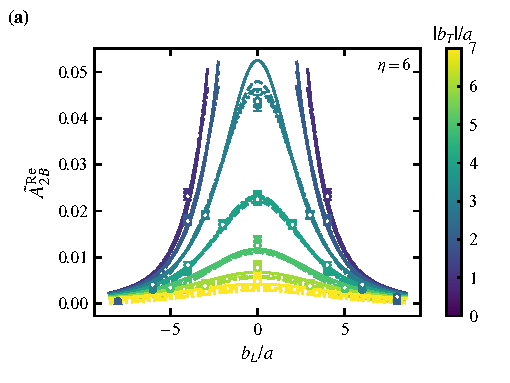
\includegraphics[width=\panelw]{figures/panels/pysr/bench_eta6.pdf}\hfill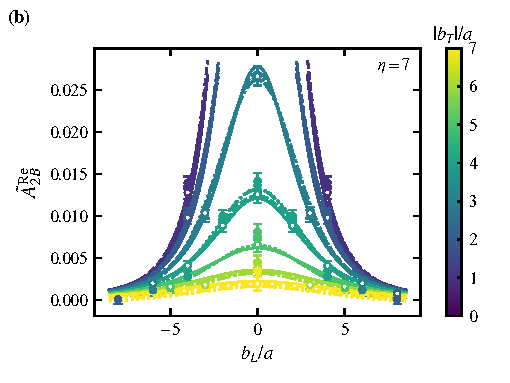
\includegraphics[width=\panelw]{figures/panels/pysr/bench_eta7.pdf}\par
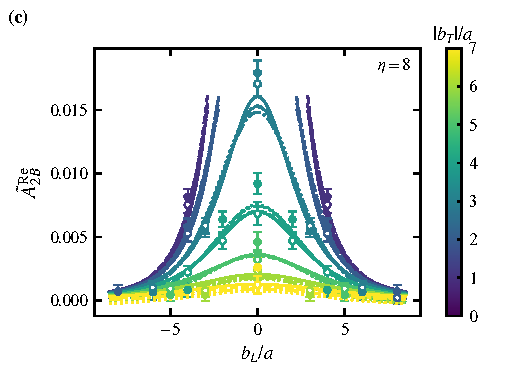
\includegraphics[width=\panelw]{figures/panels/pysr/bench_eta8.pdf}\hfill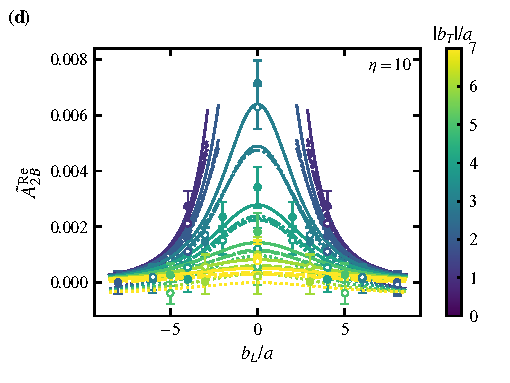
\includegraphics[width=\panelw]{figures/panels/pysr/bench_eta10.pdf}\par

\includegraphics[width=\panelw]{figures/panels/pysr/bench_legend.pdf}
\caption{\texttt{PySR} models ($C=11,13,15,17$) against the data for $\tAmp_{2B}^{\text{Re}}$ at $\eta=6,7,8,10$ in panels (a)--(d) ($P_L=-2$, $|\vect b|\ge3a$). The exponential-$\eta$ models $C=13$, $15$ and $17$ describe the data better than the power-law model $C=11$ ($\chi^2/\text{dof}=1.59$, $1.36$, $1.24$ against $2.51$, with the parameters not subtracted from the dof). Open and filled symbols are $b_T<0$ and $b_T\ge0$; colour encodes $|b_T|/a$.}
\label{fig:pysr_benchmark}
\end{figure*}

\begin{figure*}[!t]
\centering
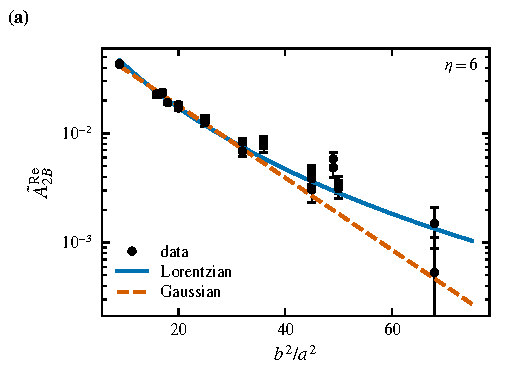
\includegraphics[width=\panelw]{figures/panels/pysr/gauss_eta6.pdf}\hfill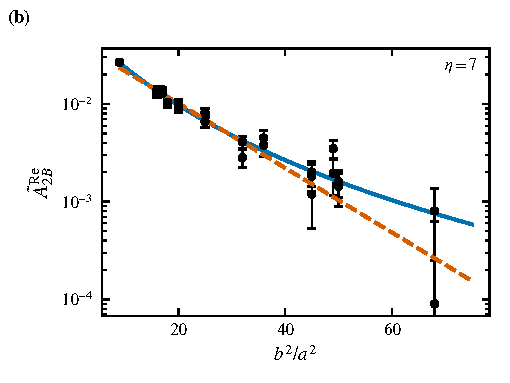
\includegraphics[width=\panelw]{figures/panels/pysr/gauss_eta7.pdf}\par
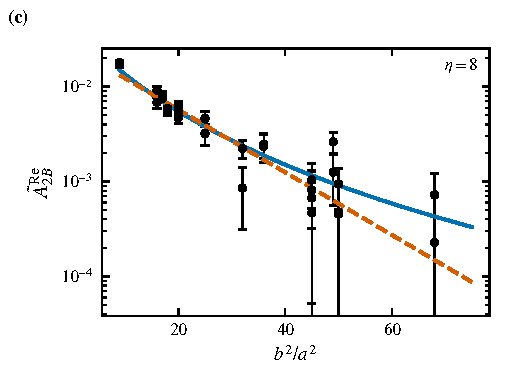
\includegraphics[width=\panelw]{figures/panels/pysr/gauss_eta8.pdf}\hfill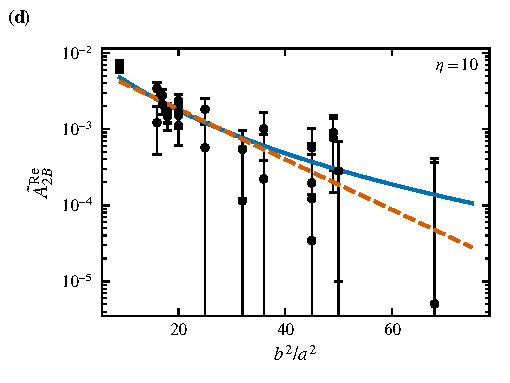
\includegraphics[width=\panelw]{figures/panels/pysr/gauss_eta10.pdf}
\caption{(a)--(d) Straight-line test at $\eta=6,7,8,10$ for a Gaussian profile at $P_L=-2$. The data (black) curve upward away from the best Gaussian fit (red dashed, $c=0.076$, $\chi^2/\text{dof}=2.03$) and follow the Lorentzian $(1+0.041\,b^2)^{-3.48}$ (blue, $\chi^2/\text{dof}=1.42$). Both fits share the factor $e^{-f\eta}$ and are fitted to all $\eta$ at once.}
\label{fig:pysr_gauss}
\end{figure*}

\subsection{Lorentzian power law and its Fourier transform}
\label{sec:power_law}

The Lorentzian power law suggested by the symbolic regression, extended by a longitudinal coefficient, reads
\begin{equation}
\tAmp_{2B}^{\text{Re}}=\frac{a\,e^{-f\eta}}{\big[1+(c+d)\,b_L^2+d\,b_T^2\big]^{j}}\,.
\label{eq:lorentzian_base}
\end{equation}
In the invariant variables the denominator is $D=[1+c\,(P\cdot b)^2/P_L^2+d\,b^2]^{j}$, which couples $(P\cdot b)^2$ and $b^2$ in one factor. This keeps the amplitude analytic at $P\cdot b=0$ and absolutely integrable over $P\cdot b$ for $j>1/2$, so the Fourier transform to $x$ exists. The coefficient $c$ determines the width of the amplitude in $P\cdot b$ and hence the width of its Fourier transform in $x$. This is the main difference from the Gaussian, whose Fourier integral requires $\alpha>\beta$ (Sec.~\ref{sec:fit_strategy}).

An exponential fall-off is a physically motivated alternative to the power law. For Euclidean quark bilinears with a straight Wilson line, the correlator at large separation is a sum of exponential decays with power-law corrections, and the mass gap is set by the binding energy of a heavy-light meson~\cite{Ji:2026asym}. That derivation does not cover staple-shaped links with $b_T\neq0$, so we test exponential decay directly on our data. A profile $e^{-c|\vect b|}$ describes $\tAmp_{2B}^{\text{Re}}$ alone about as well as the power law over $3\le|\vect b|/a\le8.2$ (Fig.~\ref{fig:exp_straight}, best fit $c=0.685$). To test exponential decay along the longitudinal direction, we apply four separable ansätze to all three amplitudes with the same $e^{-f\eta}$: a longitudinal profile $e^{-c|P\cdot b|}$ or $e^{-c(P\cdot b)^2}$ multiplying a transverse profile $e^{-d|b|}$ or $(1+db^2)^{-j}$. Table~\ref{tab:separable} compares them with the coupled power law of Eq.~\eqref{eq:lorentzian_base}. With an exponential longitudinal profile, the longitudinal coefficient of $\tAmp_{2B}^{\text{Im}}$ and $\tAmp_{12B}^{\text{Re}}$ is consistent with zero at $P_L=-1$ to $-3$ (at $P_L=-4$ only that of $\tAmp_{12B}^{\text{Re}}$ is). Without a positive $c$ the model does not decay in $P\cdot b$, and the Fourier transform to $x$ diverges. The factor $e^{-c|P\cdot b|}$ also has a cusp at $P\cdot b=0$ that conflicts with an amplitude odd in $b_L$, and at $P_L=-1$ to $-3$ $\tAmp_{2B}^{\text{Im}}$ acquires an unphysical sign. With Gaussian longitudinal profiles the global $\chi^2/\text{dof}$ is poor at $P_L=-1$ and $-2$ ($2.0$ to $2.4$) and worse than the coupled power law at $P_L=-3$ ($0.95$ against $0.71$), and the coefficient of $\tAmp_{12B}^{\text{Re}}$ is again compatible with zero. The exponential-longitudinal forms reach a lower global $\chi^2/\text{dof}$ than the coupled power law at $P_L=-1$ to $-3$, but only with a longitudinal coefficient consistent with zero or an unphysical sign of $\tAmp_{2B}^{\text{Im}}$, and at $P_L=-4$ all forms agree within errors. The coupled power law gives positive parameters for all three amplitudes and is adopted (Appendix~\ref{app:fit_exploration}).

\begin{table}
\caption{Global $\chi^2/\text{dof}$ of the four separable ansätze and the coupled power law at the four momenta (top), and key parameters at $P_L=-2$ (bottom). The key parameters at the other momenta are in Table~\ref{tab:separable_params_app}.}
\label{tab:separable}
\scriptsize
\setlength{\tabcolsep}{2pt}
\begin{ruledtabular}
\begin{tabular}{lcccc}
Ansatz & $P_L\!=\!-1$ & $-2$ & $-3$ & $-4$ \\
\hline
ExpPb\_Expb & $1.406(92)$ & $0.956(75)$ & $0.622(61)$ & $0.455(53)$ \\
ExpPb\_PowerLawb & $1.286(89)$ & $0.938(75)$ & $0.623(61)$ & $0.447(53)$ \\
GaussianPb\_Expb & $2.389(121)$ & $2.005(111)$ & $0.945(76)$ & $0.453(52)$ \\
GaussianPb\_PowerLawb & $2.316(120)$ & $1.981(111)$ & $0.948(76)$ & $0.448(52)$ \\
Coupled power law & $1.85(10)$ & $1.197(85)$ & $0.712(66)$ & $0.434(51)$ \\
\end{tabular}
\end{ruledtabular}
\medskip

\scriptsize
\begin{ruledtabular}
\begin{tabular}{lccc}
Ansatz at $P_L=-2$ & $c_{\text{im}}$ & $c_{\text{reA12B}}$ & $a_{\text{im}}$ \\
\hline
ExpPb\_Expb & $-0.001(14)$ & $0.007(14)$ & $-0.224(23)$ \\
ExpPb\_PowerLawb & $0.006(13)$ & $-0.011(16)$ & $-0.190(35)$ \\
GaussianPb\_Expb & $0.367(51)$ & $0.0021(21)$ & $+0.243(15)$ \\
GaussianPb\_PowerLawb & $0.346(43)$ & $0.0002(19)$ & $+0.249(12)$ \\
Coupled power law & $0.1346(69)$ & $0.0769(54)$ & $+0.368(12)$ \\
\end{tabular}
\end{ruledtabular}
\end{table}

\subsection{$\eta$ dependence of $c$ and $d$}
\label{sec:eta_dependence}

Guided by the \texttt{PySR} result, we explore the $\eta$ dependence of the power-law model in more detail. We fit $\tAmp_{2B}^{\text{Re}}$ with $6\le\eta\le10$ and $|\vect b|\ge3a$, using the correlated $\chi^2$ of the full Jackknife covariance matrix, and count the degrees of freedom as in the simultaneous fits, with all rows including the duplicated $b_L\to-b_L$ rows. With Eq.~\eqref{eq:lorentzian_base} and a constant $c$ we find $\chi^2/\text{dof}=1.24(15)$. An $\eta$-dependent $c$ lowers the correlated $\chi^2$ by 28 for one extra parameter, to $\chi^2/\text{dof}=1.12(14)$ for $c(1-k_1/\eta)$ (Table~\ref{tab:powerlaw_family_PL2}). A second shape parameter does not help: $c(1-k_1/\eta-k_2/\eta^2)$ has the same $\chi^2$, and $k_2=-6(25)$ is consistent with zero. The wider forms of Table~\ref{tab:powerlaw_family_PL2} also give $\chi^2/\text{dof}\approx1.12$, so the data accommodate a wide range of $\eta$ dependences of $c$, which correspond to a wide range of widths of the Fourier transform in $x$. With only the 140 independent rows, the $\chi^2/\text{dof}$ values are about 1.6 times larger, for example $1.84$ instead of $1.12$ for $c(1-k_1/\eta-k_2/\eta^2)$. For comparison, a family of Gaussian ansätze with $\eta$-dependent widths gives $\chi^2/\text{dof}$ between $1.56$ and $1.91$ (Table~\ref{tab:gauss_family_PL2}). Their correlated $\chi^2$ is 73 to 138 higher than that of the best power-law fit with the same number of parameters (for the 15 Gaussian forms that have a power-law counterpart), and for most forms their longitudinal coefficient is zero within errors or negative ($c=-0.0017(7)$ for constant $c$ and $d$).

To isolate the $\eta$ dependence of $c$ and $d$, we fix $a$, $f$ and $j$ to the values of a separate fit of each amplitude and fit the individual $\eta$ slices sequentially. We then fit a straight line $y_0+s\,(\eta-8)$ to each parameter with the full covariance across $\eta$ (Figs.~\ref{fig:c_d_eta_PL2} and~\ref{fig:c_d_eta_PL2_rest}). For $\tAmp_{2B}^{\text{Re}}$ we use the values of the global fit with $c(1-k_1/\eta-k_2/\eta^2)$ ($a=2.47$, $f=0.484$, $j=2.52$), which the other $\eta$-dependent forms of Table~\ref{tab:powerlaw_family_PL2} share closely. For $\tAmp_{12B}^{\text{Re}}$ and $\tAmp_{2B}^{\text{Im}}$ we use the values of their own global fits with constant $c$ ($a=0.77$, $f=0.50$, $j=2.41$ and $a=0.44$, $f=0.60$, $j=2.37$). For $\tAmp_{2B}^{\text{Re}}$ the parameter $c$ rises with $\eta$, with slope $0.0054(19)$ ($2.8\sigma$) and $\chi^2/\text{dof}=0.29$. The slope of $d$ is $0.0006(9)$, consistent with zero, but the line does not describe the five points ($\chi^2/\text{dof}=4.3$). Each form $c(\eta)=c\,g(\eta)$ was fitted to the five slice values of $c$ with the Jackknife covariance across $\eta$ (dashed curves in Fig.~\ref{fig:c_d_eta_PL2}, parameters in Table~\ref{tab:c_eta_forms_PL2}). A constant $c$ does not describe them ($\chi^2=8.69$ for 4 degrees of freedom), while all $\eta$-dependent forms do. Several forms describe the slice values of $c$ equally well, so goodness of fit has to be paired with the physical constraints of Sec.~\ref{sec:simultaneous_fit}. We select $c(\eta)=c\,(1-k_1/\eta-k_2/\eta^2)$, which suppresses the antiquark region $x\lesssim-0.2$ at higher momentum. We keep $d$ constant in $\eta$, although the straight line does not describe the slice values of $d$.

For $\tAmp_{12B}^{\text{Re}}$ the slopes of $c$ and $d$ are $0.0098(87)$ and $0.0004(29)$, and for $\tAmp_{2B}^{\text{Im}}$ they are $0.0010(41)$ and $-0.0006(29)$. All four are within $1.2\sigma$ of zero, with $\chi^2/\text{dof}<1$ for every line. The data for these two amplitudes are noisier. We keep $c$ and $d$ constant in $\eta$ for both.
\begin{figure*}[!t]
\centering
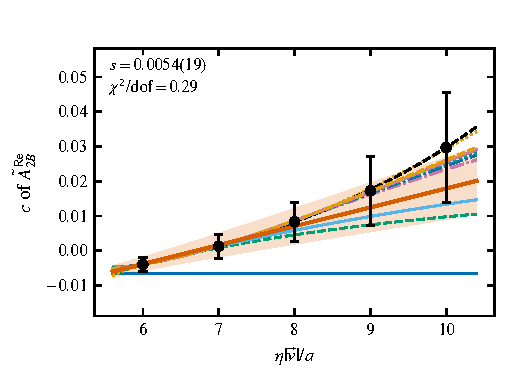
\includegraphics[width=\panelw]{figures/panels/cd/cd_ReA2B_c.pdf}\hfill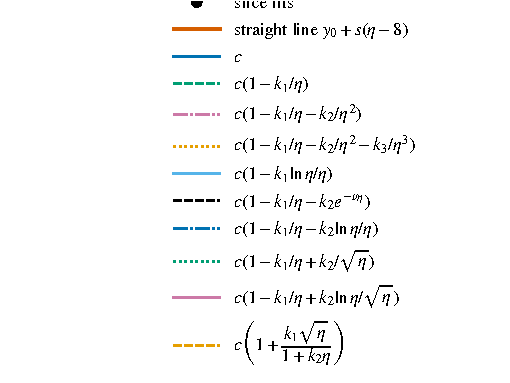
\includegraphics[width=\panelw]{figures/panels/cd/cd_legend.pdf}
\caption{Parameter $c$ of $\tAmp_{2B}^{\text{Re}}$ from fits to individual $\eta$ slices (points, diagonal Jackknife errors), with a straight-line fit $y_0+s\,(\eta-8)$ (full covariance across $\eta$, band $1\sigma$) and the forms $c(\eta)=c\,g(\eta)$ of the legend fitted to the five points (dashed curves, Table~\ref{tab:c_eta_forms_PL2}). Each panel gives the slope $s$ and the $\chi^2/\text{dof}$ of the line (3 degrees of freedom).}
\label{fig:c_d_eta_PL2}
\end{figure*}
\begin{figure*}[!t]
\centering
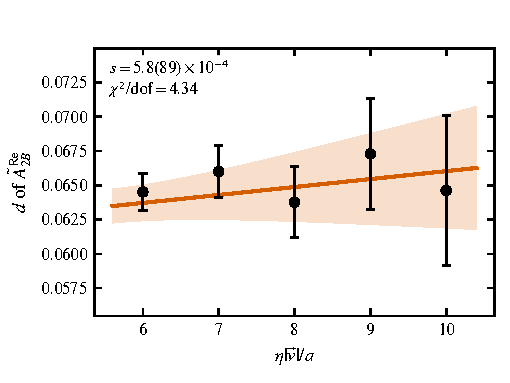
\includegraphics[width=\panelw]{figures/panels/cd/cd_ReA2B_d.pdf}\hfill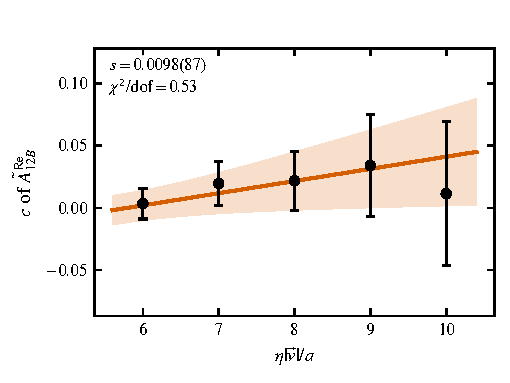
\includegraphics[width=\panelw]{figures/panels/cd/cd_ReA12B_c.pdf}\\[1ex]
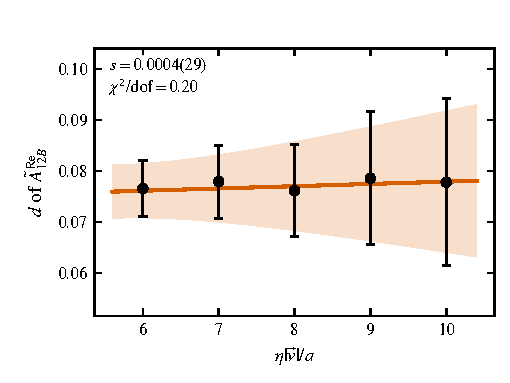
\includegraphics[width=\panelw]{figures/panels/cd/cd_ReA12B_d.pdf}\hfill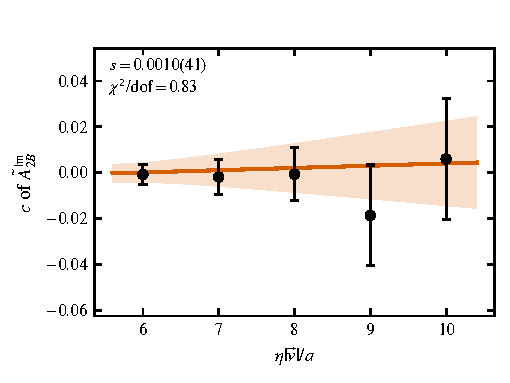
\includegraphics[width=\panelw]{figures/panels/cd/cd_ImA2B_c.pdf}\\[1ex]
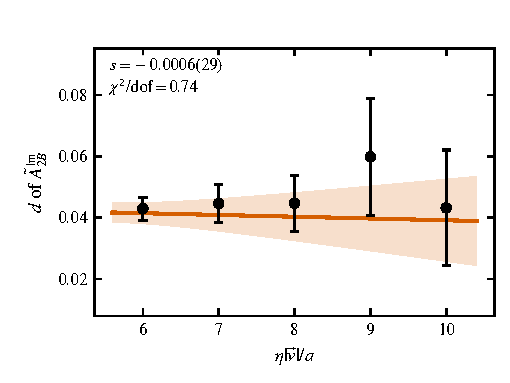
\includegraphics[width=\panelw]{figures/panels/cd/cd_ImA2B_d.pdf}
\caption{As Fig.~\ref{fig:c_d_eta_PL2}, in reading order for $d$ of $\tAmp_{2B}^{\text{Re}}$, $c$ and $d$ of $\tAmp_{12B}^{\text{Re}}$, and $c$ and $d$ of $\tAmp_{2B}^{\text{Im}}$.}
\label{fig:c_d_eta_PL2_rest}
\end{figure*}

\subsection{Simultaneous fit}
\label{sec:simultaneous_fit}

The final models are
\begin{align}
\tAmp_{2B}^{\text{Re}}&=\frac{a\,e^{-f\eta}}{\big[1+\big(d+c\,(1-\tfrac{k_1}{\eta}-\tfrac{k_2}{\eta^2})\big)b_L^2+d\,b_T^2\big]^{j}}\,,\label{eq:model_ReA2B}\\
\tAmp_{2B}^{\text{Im}}&=\frac{a''\,b_L\,e^{-f\eta}}{\big[1+(c''+d'')b_L^2+d''b_T^2\big]^{j''}}\,,\label{eq:model_ImA2B}\\
\tAmp_{12B}^{\text{Re}}&=\frac{-a'\,e^{-f\eta}}{\big[1+(c'+d')b_L^2+d'b_T^2\big]^{j'}}\,.\label{eq:model_ReA12B}
\end{align}
The choice of $c(\eta)$ for $\tAmp_{2B}^{\text{Re}}$ among candidates with equal $\chi^2/\text{dof}$ combines the fit quality with two physical requirements: the antiquark region $x\lesssim-0.2$ of $\tilde f_1^{(0)}=2\tAmp_{2B}^{[x]}$ must be suppressed, which involves both $\tAmp_{2B}^{\text{Re}}$ and $\tAmp_{2B}^{\text{Im}}$, and the $x$-integrated results must agree with earlier first-moment calculations~\cite{Musch:2011er,Yoon:2017qzo}. % TODO(Hari): the boundary x=-0.2 is a physics criterion, not a computed value; no script in the repo derives it (python_fits/paper_numbers lists it as not reproducible)

The three amplitude models share an $\eta$ dependence damped by a common exponential factor $e^{-f\eta}$. Because the Sivers shift is a ratio, this factor, which does not depend on the integration variable $P\cdot b$, cancels between the numerator and the denominator of Eq.~\eqref{eq:sivers_shift_xdep}. We enforce this shared $\eta$ dependence with a simultaneous global fit at each momentum in which $f$ is the same in all three amplitudes, which reduces the number of free parameters. The amplitudes are extracted from the same gauge field configurations at nearby coordinates $(b_L,b_T,\eta)$, so their statistical fluctuations are correlated and an uncorrelated $\chi^2$ would weight the points incorrectly. We therefore minimize the correlated $\chi^2$ with the full Jackknife covariance matrix~\cite{Boram2011Covariance}, which includes correlations between different $(b_L,b_T,\eta)$ points and between the three amplitudes, using \texttt{lsqfit}~\cite{Lepage:2001ym}. The global $\chi^2/\text{dof}$ is $1.85(10)$, $1.197(85)$, $0.712(66)$ and $0.434(51)$ for $P_L=-1,\ldots,-4$.

\begin{table}
\caption{Parameters of the simultaneous fit at $P_L=-2$ ($|\vect b|\ge3a$, $6\le\eta\le10$) with a common $f$. Global $\chi^2/\text{dof}=1.197(85)$. The parameters of $\tAmp_{2B}^{\text{Im}}$ are $a'',c'',d'',j''$ and those of $\tAmp_{12B}^{\text{Re}}$ are $a',c',d',j'$ in Eqs.~\eqref{eq:model_ImA2B} and~\eqref{eq:model_ReA12B}.}
\label{tab:fit_params_P2}
\small
\begin{ruledtabular}
\begin{tabular}{lccc}
 & $\tAmp_{2B}^{\text{Re}}$ & $\tAmp_{2B}^{\text{Im}}$ & $\tAmp_{12B}^{\text{Re}}$ \\
\hline
$a$ & $3.9833(80)$ & $0.368(12)$ & $0.632(19)$ \\
$c$ & $0.166(35)$ & $0.1346(69)$ & $0.0769(54)$ \\
$d$ & $0.1020(46)$ & $0.1305(67)$ & $0.0741(52)$ \\
$k_1$ & $12.305(14)$ & --- & --- \\
$k_2$ & $-36.1919(27)$ & --- & --- \\
$j$ & $2.061(20)$ & $1.141(20)$ & $2.0141(69)$ \\
$f$ & \multicolumn{3}{c}{$0.5357(66)$ (common)} \\
\end{tabular}
\end{ruledtabular}
\end{table}

Table~\ref{tab:fit_params_P2} gives the parameters and the global $\chi^2/\text{dof}$ at $P_L=-2$. Figs.~\ref{fig:ft_xdep_P2}--\ref{fig:ft_xdep_P2_siv} show the $x$ dependence at $b^2=9a^2$ obtained from the Fourier transform of the fitted amplitudes over $P\cdot b$.


\begin{figure*}[!t]
\centering
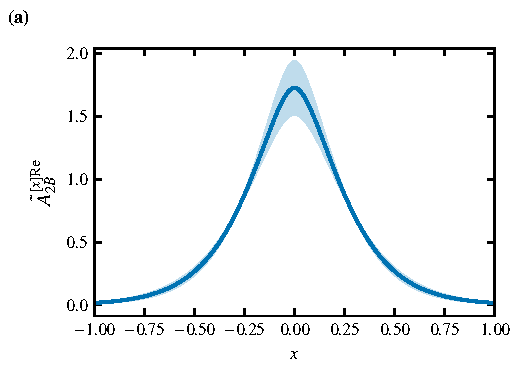
\includegraphics[width=\panelw]{figures/panels/xdep/xdep_PL2_ReA2B.pdf}\hfill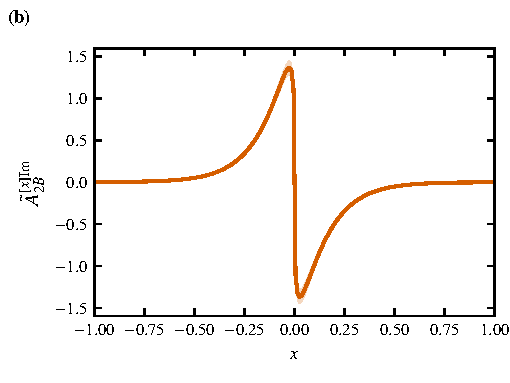
\includegraphics[width=\panelw]{figures/panels/xdep/xdep_PL2_ImA2B.pdf}
\caption{$x$ dependence at $b^2=9a^2$ of the Fourier transforms $\tAmp^{[x]\text{Re}}_{2B}$ (a) and $\tAmp^{[x]\text{Im}}_{2B}$ (b) at $P_L=-2$. Bands are Jackknife uncertainties.}
\label{fig:ft_xdep_P2}
\end{figure*}
\begin{figure*}[!t]
\centering
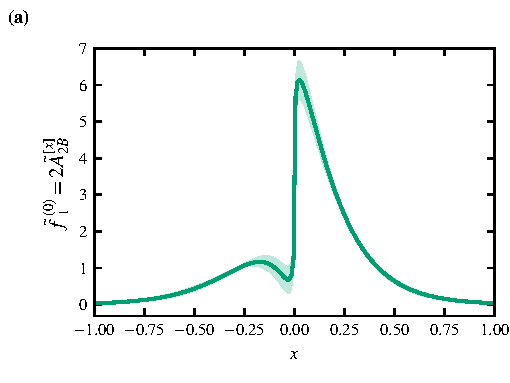
\includegraphics[width=\panelw]{figures/panels/xdep/xdep_PL2_f1.pdf}\hfill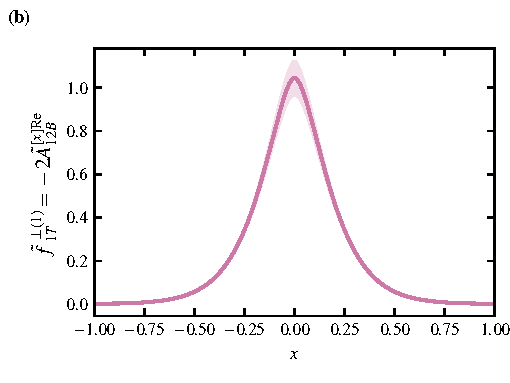
\includegraphics[width=\panelw]{figures/panels/xdep/xdep_PL2_f1T.pdf}
\caption{As Fig.~\ref{fig:ft_xdep_P2}, for $\tilde f_1^{(0)}=2\tAmp^{[x]}_{2B}$ (a) and $\tilde f_{1T}^{\perp(1)}=-2\tAmp^{[x]\text{Re}}_{12B}$ (b).}
\label{fig:ft_xdep_P2_tmd}
\end{figure*}
\begin{figure*}[!t]
\centering
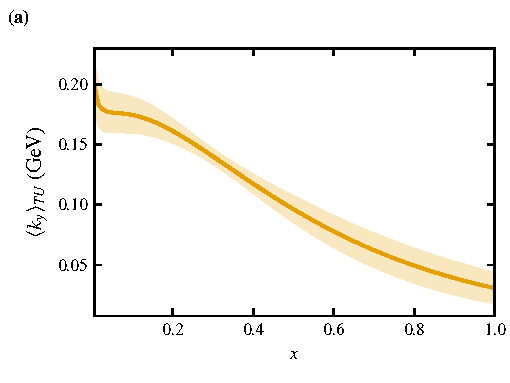
\includegraphics[width=\panelw]{figures/panels/xdep/xdep_PL2_ky.pdf}\hfill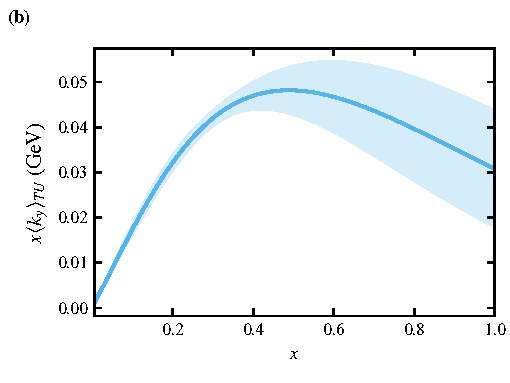
\includegraphics[width=\panelw]{figures/panels/xdep/xdep_PL2_xky.pdf}
\caption{As Fig.~\ref{fig:ft_xdep_P2}, for the Sivers shift $\langle k_y\rangle_{TU}$ (a) and $x\langle k_y\rangle_{TU}$ (b).}
\label{fig:ft_xdep_P2_siv}
\end{figure*}
